\twocolumn[\begin{@twocolumnfalse}
	\chapter{Freeing a stuck fan\hskip0.5cm\difficulty{2}}
	In many `New Old Stock' (NOS) NABU Personal Computers the fan either doesn't spin freely or is completely stuck. Several fixes have been suggested, including bending fan blades or filing down the fan tips. Following is a simpler and less destructive solution. Alternatively, the fan can be replaced following the instructions in Section \ref{sec:fan-replacement}, `Replacing the NABU fan assembly' on page \pageref{sec:fan-replacement}.
	\vskip1em
\end{@twocolumnfalse}]
\section{Removing the fan}
\awesomebox[red]{2pt}{\faBolt}{red}{To prevent electric shock, you \textbf{must} disconnect your NABU Personal Computer from mains power before removing the system cover!}
\begin{enumerate}
	\item Remove the outer computer cover by undoing the screws on either side of your NABU system. This will expose the main system board (right) and power supply bay (left).
	\item Remove the cover over the power supply by undoing the two screws on the right-hand side and lifting the cover upwards.
	\item Undo the 4 bolts that hold the fan assembly in place and free the fan such that the 3 adjustment screws are accessible (see Figure \ref{fig:fanassembly}).
\end{enumerate}
\section{Adjusting the fan assembly}
\begin{enumerate}
	\item Loosen the screws and gently adjust the blade assembly until the fan blades spin freely, then re-tighten the screws. Repeat as necessary.
\end{enumerate}
\section{Re-installing the fan}
\begin{enumerate}
	\item Place the fan back into the system such that the adjustment screws are facing outwards. Then fix in place using the 4 nuts and bolts from step 1.1.3.
	\item Check that there are no loose parts, then replace the NABU PSU cover and fix in place with its 2 screws.
	\item Replace the NABU system cover, securing it with 4 screws.
\end{enumerate}
\newpage
\begin{figure}[h!]
	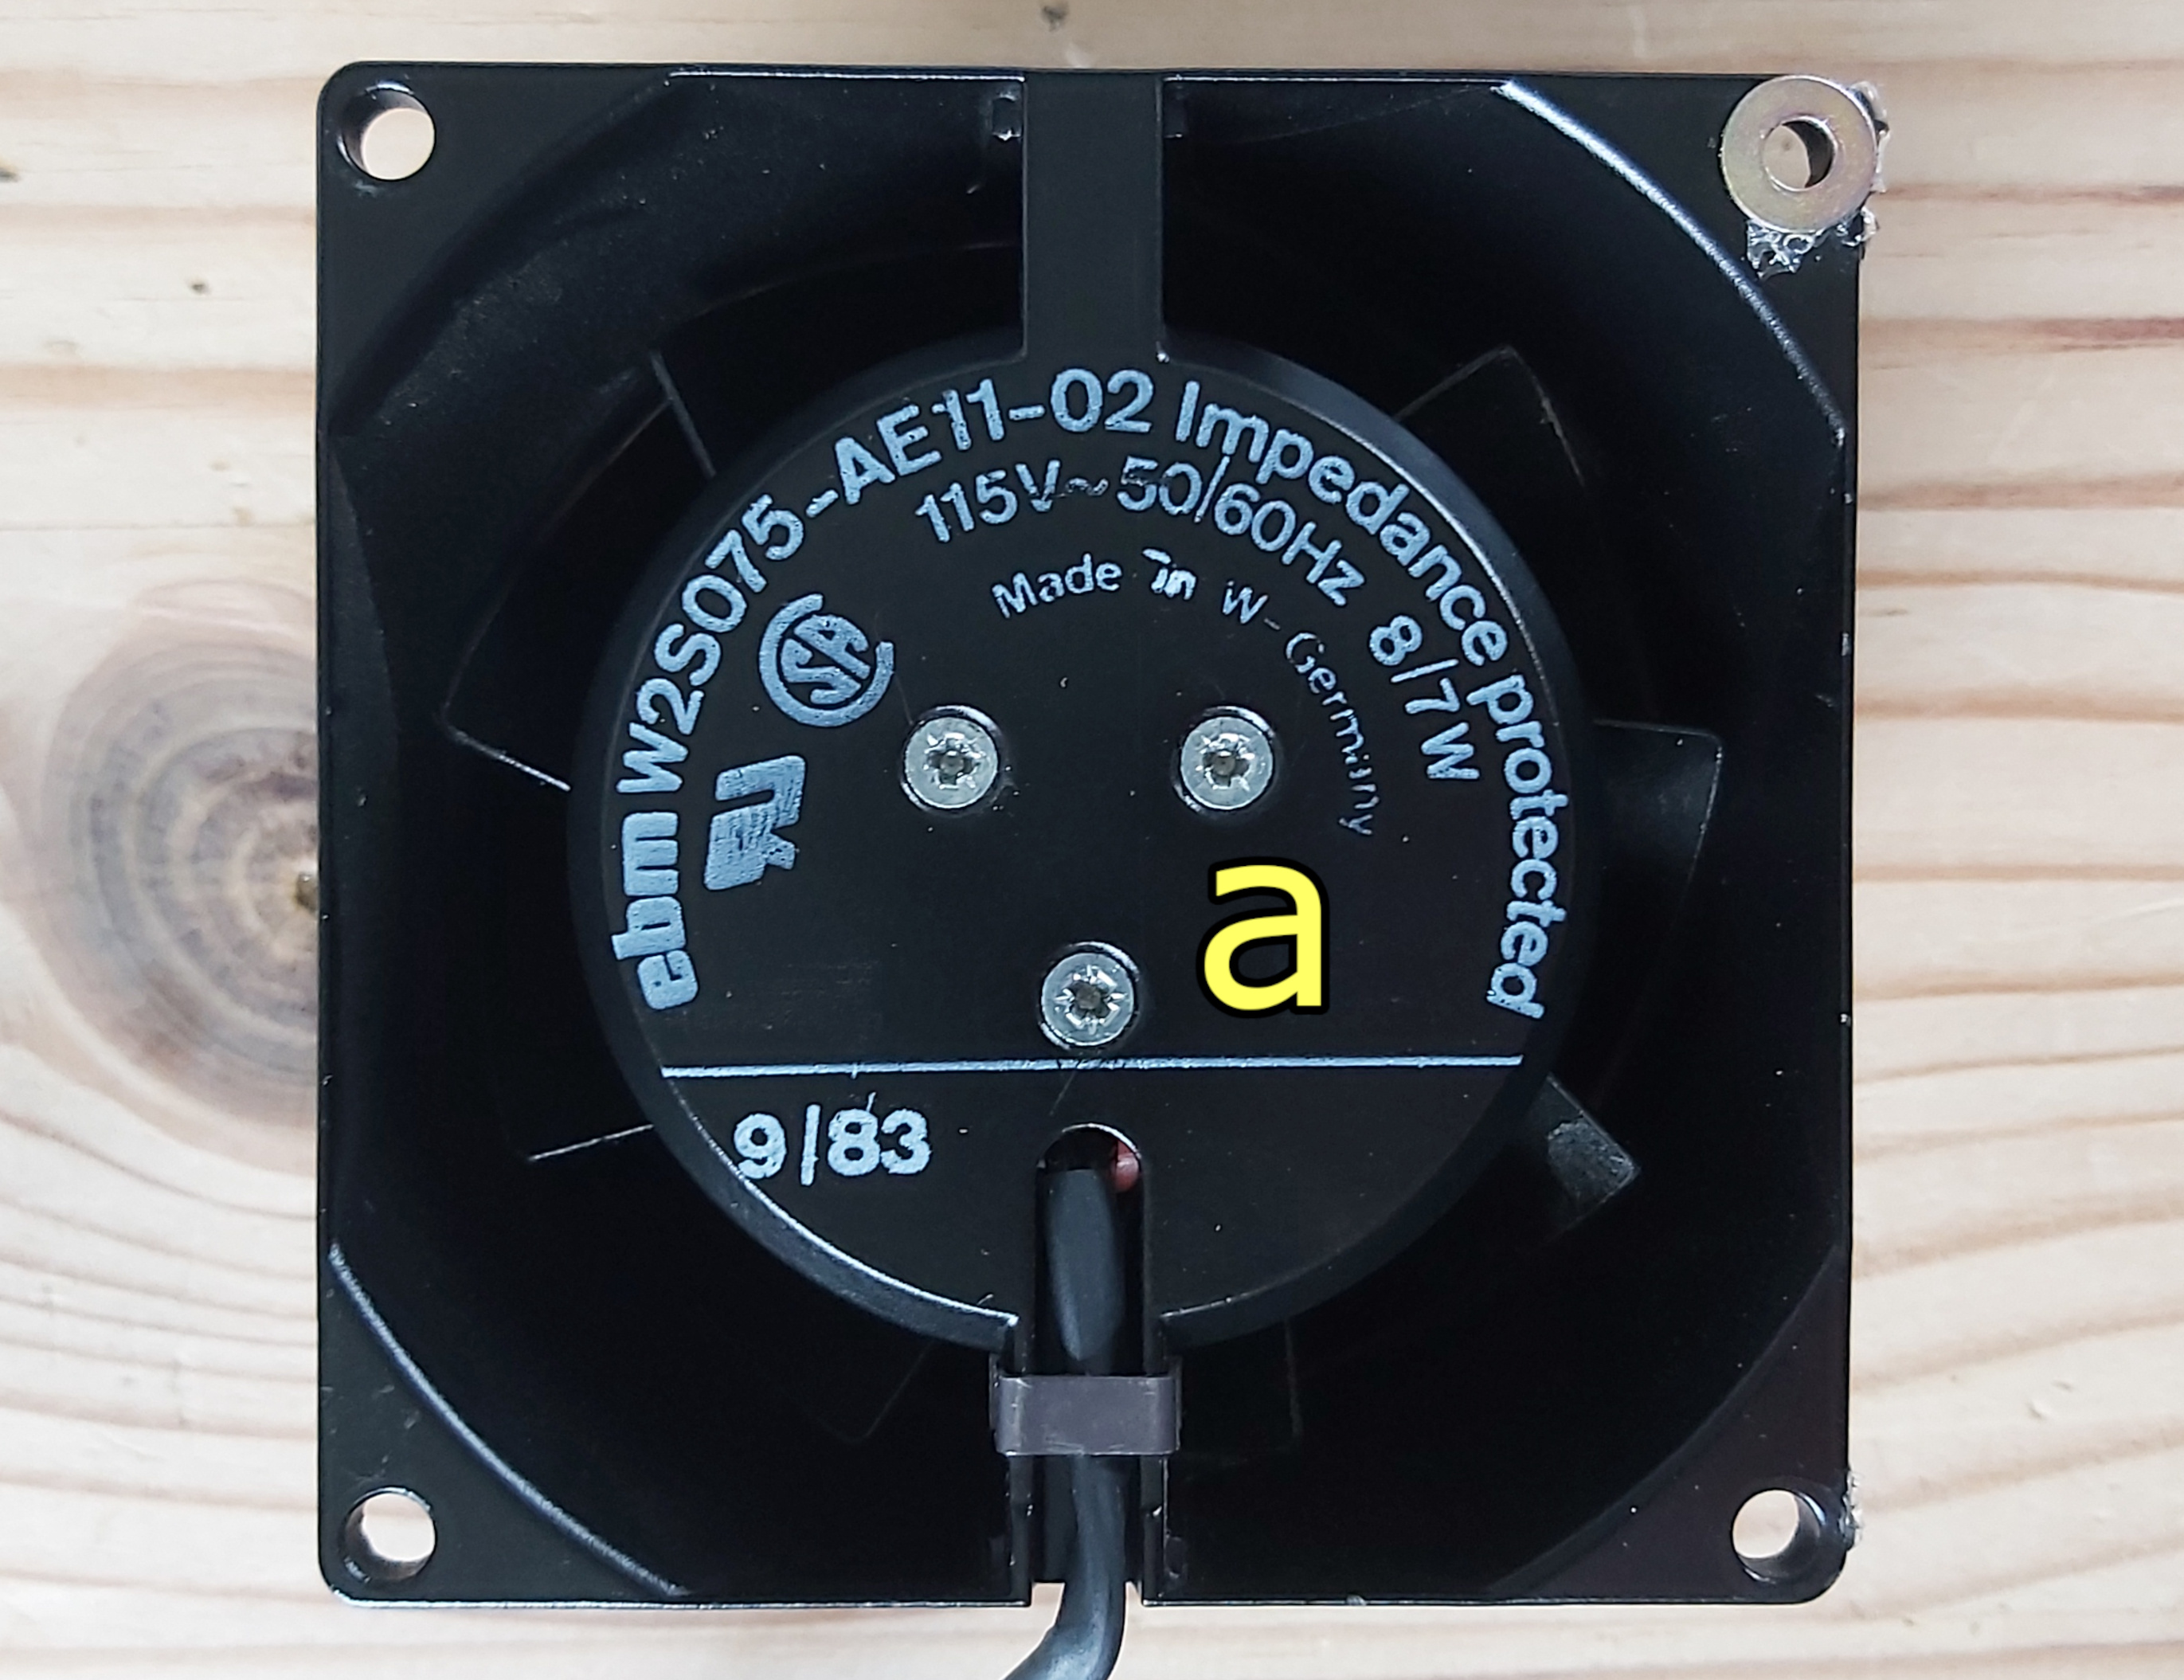
\includegraphics[width=\columnwidth]{images/fan-image-1.jpg}
	\caption{Adjust the blade assembly screws.}
	\label{fig:fanassembly}
\end{figure}
